\begin{frame}
  \frametitle{Surveys and solutions}
  \begin{block}{Talks and papers}
    \begin{itemize}
      \item Ristic: BlackHat 2010
      \item EFF: Defcon 2010
      \item Vratonjic et al., WPES, 2011
      \item Holz et al., IMC, 2011
    \end{itemize}
  \end{block}
  \begin{block}{They all agree: the system does not work, although some apologists remain.}\end{block}
\end{frame}


\begin{frame}
\frametitle{No silver bullet}
  \begin{block}{Scope of SSL/TLS:}
    \begin{itemize}
      \item Originally meant to protect things like credit card numbers
      \item State-scale attacks were not in scope back in the 1990s
    \end{itemize}
  \end{block}
  \begin{block}{Some proposals}
    \begin{itemize}
      \item Notary principle: Perspectives, Convergence
      \item Public Logs: Sovereign Keys, Certificate Transparency
      \item Keys in DNS(SEC): DANE, CAA
      \item Pinning
      \item PKI-me-harder
    \end{itemize}
  \end{block}
\end{frame}

\begin{frame}
  \frametitle{Errors in TLS Connection Setup}
  \begin{block}{Scans from Germany, Nov 2009 and Apr 2011}
    \begin{figure}
    \centering
      \includegraphics[scale=1.2]{plots/conn-err.pdf}
    \end{figure}
  \end{block}
\end{frame}


\begin{frame}
  \frametitle{Errors in TLS Connection Setup}
  \begin{block}{\texttt{UNKNOWN PROTOCOL}}
    \begin{itemize}
      \item Rescanned those hosts and manual sampling
      \item Always plain HTTP...
      \item ... and always an \texttt{index.html} with HTML 2 ...
      \item Hypothesis: old servers, old configurations
      \item More likely to happen in the lower ranks
    \end{itemize}
  \end{block}
\end{frame}

\begin{frame}
  \frametitle{Unusual Host Names}
  \begin{block}{CN=plesk or similar}
   \begin{itemize}
      \item Found in 7.3\% of certificates
      \item Verified: Plesk/Parallels panels
%       \item Verified: rescanned,  histograms of HTML replies
   \end{itemize}
  \end{block}
  \begin{block}{CN=localhost}
    \begin{itemize}
      \item 4.7\% of certificates
%       \item Very common: redirection to HTTP after HTTPs
    \end{itemize}
  \end{block}
\end{frame}


\begin{frame}
  \frametitle{Symmetric Ciphers}
  \begin{block}{Results from monitoring}
    \begin{figure}
    \centering
      \includegraphics[scale=.85]{plots/top-ciphers.pdf}
    \end{figure}
  \end{block}
  \begin{block}{(Mostly) in line with results from 2007 by Lee et al.}
   \begin{itemize}
    \item Order of AES and RC4 has shifted, RC4-128 most popular
   \end{itemize}
  \end{block}
\end{frame}


\begin{frame}
  \frametitle{Debian Weak Keys}
  \begin{block}{Weak randomness in key generation \\-- serious bug of 2008}
    \begin{figure}
    \centering
     \includegraphics[scale=.8]{plots/debian-weak-keys.pdf}
    \end{figure}
  \end{block}
  \begin{block}{In line with findings of 2009 by Yilek et al.}\end{block}
\end{frame}

\begin{frame}
  \frametitle{Public Key Lengths}
  \begin{block}{CDF for RSA key lengths -- linear Y axis}
    \begin{figure}
    \centering
     \includegraphics[scale=1.2]{plots/keylengths-times-linY.pdf}
    \end{figure}
  \end{block}
\end{frame}



\begin{frame}
  \frametitle{Public Key Lengths}
  \begin{block}{CDF for RSA key lengths -- double-log Y axis}
     \begin{figure}
    \centering
     \includegraphics[scale=1.2]{plots/keylengths-times-logY.pdf}
    \end{figure}
  \end{block}
\end{frame}



\begin{frame}
  \frametitle{Certificate Occurrences}
  \begin{block}{Most frequent Common Name occurrences}
    \begin{figure}
    \centering
      \includegraphics[scale=1.4]{plots/top-domains.pdf}
    \end{figure}
  \end{block}
\end{frame}



\begin{frame}
  \frametitle{Certificate Chains}
  \vskip -1.5cm
  \begin{block}{}
    \begin{figure}
      \centering
      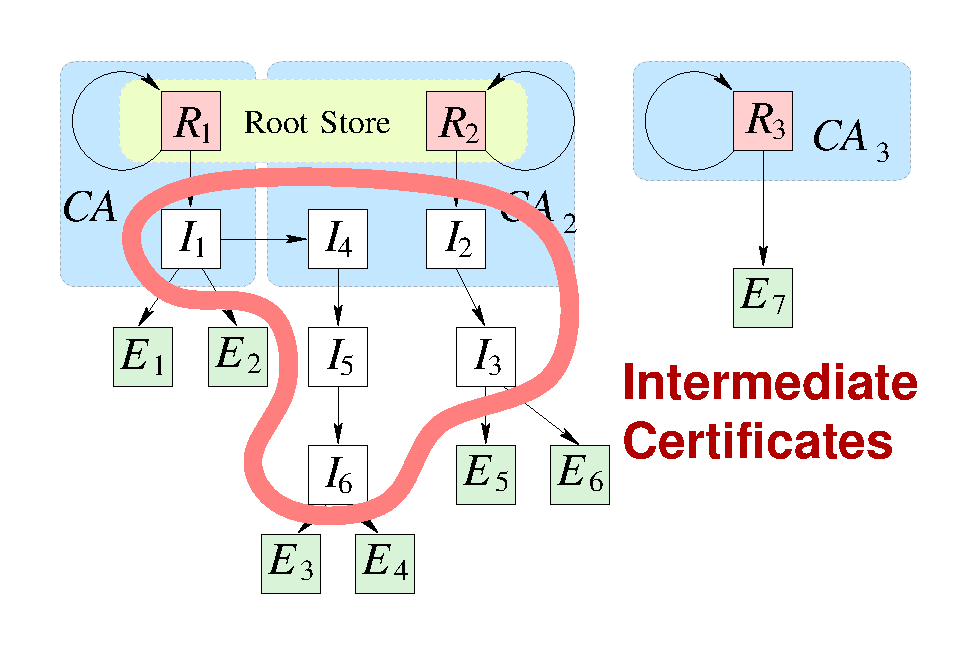
\includegraphics[scale=.7]{figures/x509tree-inter.pdf}
    \end{figure}
  \end{block}
\end{frame}




\begin{frame}
  \frametitle{Certificate Chain Lengths}
%   \vskip -1cm
%   \begin{columns}
%   \column{.5\textwidth}
    \begin{figure}
    \centering
      \includegraphics[scale=.9]{plots/chain-lengths.pdf}
    \end{figure}
%   \column{.5\textwidth}
%     \begin{figure}
%     \centering
%       \includegraphics[scale=.75]{plots/certchains-and-intermediates.pdf}
%     \end{figure}
%   \end{columns}
  \begin{block}{Finding more positive than negative:}
    \begin{itemize}
      \item Trend to use intermediate certificates more often
      \item Allows to keep Root Certificates offline
      \item But chains still reasonably short
   \end{itemize}
  \end{block}
\end{frame}

\begin{frame}
  \frametitle{Certificate Issuers}
  \begin{block}{Very few CAs account for $>$ 50\% of certificates}
    \begin{figure}
    \centering
     \includegraphics[scale=1]{plots/top-issuers.pdf}
    \end{figure}
  \end{block}
  \begin{block}{But there are 150+ Root Certificates in Mozilla.}\end{block}
\end{frame}
